% Neural network diagram
% Made with Xematics. Positions are in px (1 px = 0.75 pt), as in the SVG export.
\documentclass[tikz, border=4pt]{standalone}
\usetikzlibrary{arrows.meta}
\definecolor{xm1}{HTML}{FFFFFF}
\definecolor{xm2}{HTML}{6B7280}
\definecolor{xm3}{HTML}{D4E8F5}
\definecolor{xm4}{HTML}{0072B2}
\definecolor{xm5}{HTML}{F1F2F4}
\definecolor{xm6}{HTML}{4B5563}
\definecolor{xm7}{HTML}{FBE8C4}
\definecolor{xm8}{HTML}{B97800}
\definecolor{xm9}{HTML}{1F2937}
\begin{document}
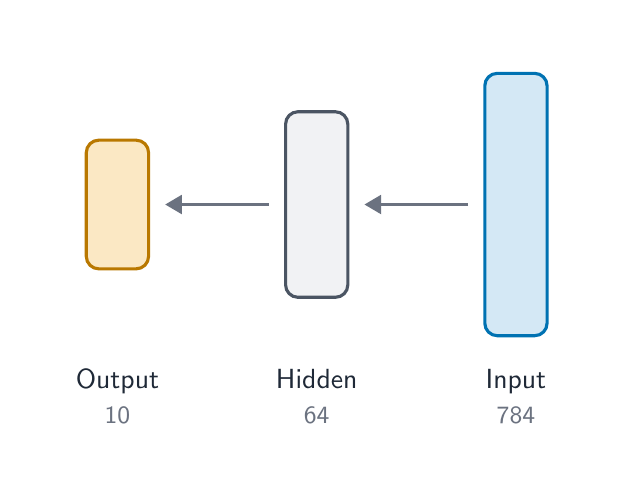
\begin{tikzpicture}[x=0.75pt, y=-0.75pt]
  \tikzset{
    xm arrow/.style={draw=xm2, line width=1.05pt, -{Triangle[length=6pt, width=6.75pt]}},
    xm box input/.style={fill=xm3, draw=xm4, line width=1.13pt, rounded corners=4.5pt},
    xm box hidden/.style={fill=xm5, draw=xm6, line width=1.13pt, rounded corners=4.5pt},
    xm box output/.style={fill=xm7, draw=xm8, line width=1.13pt, rounded corners=4.5pt},
    xm name xm9/.style={text=xm9, inner sep=0, font=\sffamily\fontsize{9.75}{11.7}\selectfont},
    xm size xm2/.style={text=xm2, inner sep=0, font=\sffamily\fontsize{9}{10.8}\selectfont},
  }
  \fill[xm1] (0,0) rectangle (273.07,215.66);
  % Connections 0
  \draw[xm arrow] (212.25,85.2) -- (162.25,85.2);
  % Connections 1
  \draw[xm arrow] (116.25,85.2) -- (66.25,85.2);
  % Layers
  \draw[xm box input] (220.25,22) rectangle ++(30,126.41);
  \draw[xm box hidden] (124.25,40.5) rectangle ++(30,89.41);
  \draw[xm box output] (28.25,54.2) rectangle ++(30,62);
  % Labels
  \node[xm name xm9, anchor=base] at (235.25,174) {Input};
  \node[xm size xm2, anchor=base] at (235.25,190.76) {784};
  \node[xm name xm9, anchor=base] at (139.25,174) {Hidden};
  \node[xm size xm2, anchor=base] at (139.25,190.76) {64};
  \node[xm name xm9, anchor=base] at (43.25,174) {Output};
  \node[xm size xm2, anchor=base] at (43.25,190.76) {10};
\end{tikzpicture}
\end{document}
